\documentclass[handout]{ximera}

\usepackage{pgf,tikz}
\usepackage{mathrsfs}
\usetikzlibrary{shapes,arrows}
\usepackage{framed}
\pgfplotsset{compat=1.13}

\graphicspath{
  {./}
  {ximeraTutorial/}
}

\newenvironment{sectionOutcomes}{}{}


% Below is the preamble from the textbook in /laode, by Golubitsky and Dellnitz
% ... with problematic stuff commented out
% Followed by the hw-preamble from worksheet-builder

%\usepackage{ulem}
\usepackage[normalem]{ulem}

\epstopdfsetup{outdir=./}

\usepackage{morewrites}
\makeatletter
\newcommand\subfile[1]{%
\renewcommand{\input}[1]{}%
\begingroup\skip@preamble\otherinput{#1}\endgroup\par\vspace{\topsep}
\let\input\otherinput}
\makeatother

\newcommand{\EXER}{}
\newcommand{\includeexercises}{\EXER\directlua{dofile(kpse.find_file("exercises","lua"))}}

\newenvironment{computerExercise}{\begin{exercise}}{\end{exercise}}

%\newcounter{ccounter}
%\setcounter{ccounter}{1}
%\newcommand{\Chapter}[1]{\setcounter{chapter}{\arabic{ccounter}}\chapter{#1}\addtocounter{ccounter}{1}}

%\newcommand{\section}[1]{\section{#1}\setcounter{thm}{0}\setcounter{equation}{0}}

%\renewcommand{\theequation}{\arabic{chapter}.\arabic{section}.\arabic{equation}}
%\renewcommand{\thefigure}{\arabic{chapter}.\arabic{figure}}
%\renewcommand{\thetable}{\arabic{chapter}.\arabic{table}}

%\newcommand{\Sec}[2]{\section{#1}\markright{\arabic{ccounter}.\arabic{section}.#2}\setcounter{equation}{0}\setcounter{thm}{0}\setcounter{figure}{0}}
  
\newcommand{\Sec}[2]{\section{#1}}

\setcounter{secnumdepth}{2}
%\setcounter{secnumdepth}{1} 

%\newcounter{THM}
%\renewcommand{\theTHM}{\arabic{chapter}.\arabic{section}}

\newcommand{\trademark}{{R\!\!\!\!\!\bigcirc}}
%\newtheorem{exercise}{}

\newcommand{\dfield}{{\sf SlopeField}}

\newcommand{\pplane}{{\sf PhasePlane}}

\newcommand{\PPLANE}{{\sf PHASEPLANE}}

% BADBAD: \newcommand{\Bbb}{\bf}. % Package amsfonts Warning: Obsolete command \Bbb; \mathbb should be used instead.

\newcommand{\R}{\mbox{$\mathbb{R}$}}
\let\C\relax
\newcommand{\C}{\mbox{$\mathbb{C}$}}
\newcommand{\Z}{\mbox{$\mathbb{Z}$}}
\newcommand{\N}{\mbox{$\mathbb{N}$}}
\newcommand{\D}{\mbox{{\bf D}}}

\newcommand{\WW}{\mathcal{W}}

\usepackage{amssymb}
%\newcommand{\qed}{\hfill\mbox{\raggedright$\square$} \vspace{1ex}}
%\newcommand{\proof}{\noindent {\bf Proof:} \hspace{0.1in}}

\newcommand{\setmin}{\;\mbox{--}\;}
\newcommand{\Matlab}{{M\small{AT\-LAB}} }
\newcommand{\Matlabp}{{M\small{AT\-LAB}}}
\newcommand{\computer}{\Matlab Instructions}
\renewcommand{\computer}{M\small{ATLAB} Instructions}
\newcommand{\half}{\mbox{$\frac{1}{2}$}}
\newcommand{\compose}{\raisebox{.15ex}{\mbox{{\scriptsize$\circ$}}}}
\newcommand{\AND}{\quad\mbox{and}\quad}
\newcommand{\vect}[2]{\left(\begin{array}{c} #1_1 \\ \vdots \\
 #1_{#2}\end{array}\right)}
\newcommand{\mattwo}[4]{\left(\begin{array}{rr} #1 & #2\\ #3
&#4\end{array}\right)}
\newcommand{\mattwoc}[4]{\left(\begin{array}{cc} #1 & #2\\ #3
&#4\end{array}\right)}
\newcommand{\vectwo}[2]{\left(\begin{array}{r} #1 \\ #2\end{array}\right)}
\newcommand{\vectwoc}[2]{\left(\begin{array}{c} #1 \\ #2\end{array}\right)}

\newcommand{\ignore}[1]{}


\newcommand{\inv}{^{-1}}
\newcommand{\CC}{{\cal C}}
\newcommand{\CCone}{\CC^1}
\newcommand{\Span}{{\rm span}}
\newcommand{\rank}{{\rm rank}}
\newcommand{\trace}{{\rm tr}}
\newcommand{\RE}{{\rm Re}}
\newcommand{\IM}{{\rm Im}}
\newcommand{\nulls}{{\rm null\;space}}

\newcommand{\dps}{\displaystyle}
\newcommand{\arraystart}{\renewcommand{\arraystretch}{1.8}}
\newcommand{\arrayfinish}{\renewcommand{\arraystretch}{1.2}}
\newcommand{\Start}[1]{\vspace{0.08in}\noindent {\bf Section~\ref{#1}}}
\newcommand{\exer}[1]{\noindent {\bf \ref{#1}}}
\newcommand{\ans}{\textbf{Answer:} }
\newcommand{\matthree}[9]{\left(\begin{array}{rrr} #1 & #2 & #3 \\ #4 & #5 & #6
\\ #7 & #8 & #9\end{array}\right)}
\newcommand{\cvectwo}[2]{\left(\begin{array}{c} #1 \\ #2\end{array}\right)}
\newcommand{\cmatthree}[9]{\left(\begin{array}{ccc} #1 & #2 & #3 \\ #4 & #5 &
#6 \\ #7 & #8 & #9\end{array}\right)}
\newcommand{\vecthree}[3]{\left(\begin{array}{r} #1 \\ #2 \\
#3\end{array}\right)}
\newcommand{\cvecthree}[3]{\left(\begin{array}{c} #1 \\ #2 \\
#3\end{array}\right)}
\newcommand{\cmattwo}[4]{\left(\begin{array}{cc} #1 & #2\\ #3
&#4\end{array}\right)}

\newcommand{\Matrix}[1]{\ensuremath{\left(\begin{array}{rrrrrrrrrrrrrrrrrr} #1 \end{array}\right)}}

\newcommand{\Matrixc}[1]{\ensuremath{\left(\begin{array}{cccccccccccc} #1 \end{array}\right)}}



\renewcommand{\labelenumi}{\theenumi}
\newenvironment{enumeratea}%
{\begingroup
 \renewcommand{\theenumi}{\alph{enumi}}
 \renewcommand{\labelenumi}{(\theenumi)}
 \begin{enumerate}}
 {\end{enumerate}
 \endgroup}

\newcounter{help}
\renewcommand{\thehelp}{\thesection.\arabic{equation}}

%\newenvironment{equation*}%
%{\renewcommand\endequation{\eqno (\theequation)* $$}%
%   \begin{equation}}%
%   {\end{equation}\renewcommand\endequation{\eqno \@eqnnum
%$$\global\@ignoretrue}}

\author{Martin Golubitsky and Michael Dellnitz}

%\newenvironment{matlabEquation}%
%{\renewcommand\endequation{\eqno (\theequation*) $$}%
%   \begin{equation}}%
%   {\end{equation}\renewcommand\endequation{\eqno \@eqnnum
% $$\global\@ignoretrue}}

\newcommand{\soln}{\textbf{Solution:} }
\newcommand{\exercap}[1]{\centerline{Figure~\ref{#1}}}
\newcommand{\exercaptwo}[1]{\centerline{Figure~\ref{#1}a\hspace{2.1in}
Figure~\ref{#1}b}}
\newcommand{\exercapthree}[1]{\centerline{Figure~\ref{#1}a\hspace{1.2in}
Figure~\ref{#1}b\hspace{1.2in}Figure~\ref{#1}c}}
\newcommand{\para}{\hspace{0.4in}}

%\usepackage{ifluatex}
%\ifluatex
%\ifcsname displaysolutions\endcsname%
%\else
%\renewenvironment{solution}{\suppress}{\endsuppress}
%\fi
%\else
%\renewenvironment{solution}{}{}
%\fi
%
%\ifcsname answer\endcsname
%\renewcommand{\answer}{}
%\fi

%\ifxake
%\newenvironment{matlabEquation}{\begin{equation}}{\end{equation}}
%\else
\newenvironment{matlabEquation}%
{\let\oldtheequation\theequation\renewcommand{\theequation}{\oldtheequation*}\begin{equation}}%
  {\end{equation}\let\theequation\oldtheequation}
%\fi

%\makeatother

\newcommand{\RED}[1]{{\color{red}{#1}}} 


%%
%%
%% Worksheet-builder preamble
%%
%%

\usepackage{xcolor}
\renewenvironment{solution}{\color{blue}}{\color{black}}
\renewenvironment{computerExercise}{\begin{exercise}\textsc{(matlab)} }{\end{exercise}}

%\usepackage{environ}
%\RenewEnviron{prompt}{}
%\RenewEnviron{hint}{}
%\RenewEnviron{multipleChoice}{}
%\RenewEnviron{feedback}{}

\renewcommand{\ans}{\noindent\textbf{Answer: }}
\renewcommand{\soln}{\noindent\textbf{Solution: }}

%\renewcommand{\answer}[2][]{#2}

% if you want to hide solutions, uncomment the following
%\usepackage{comment}\excludecomment{solution}

\def\isitmatlab{}
\newcommand{\matlab}{\def\isitmatlab{ (MATLAB)}}

\makeatletter
\newcommand{\exerciselabel}[2]{\textbf{\textsection #2, Exercise #1\isitmatlab.}\def\@currentlabel{#1}\def\isitmatlab{}}
\makeatother

\newcounter{problemx}
\newcommand{\problemlabel}{\refstepcounter{problemx}\section*{Problem \arabic{problemx}}}
\newcommand{\matlabproblemlabel}{\refstepcounter{problemx}\section*{Problem \arabic{problemx} (MATLAB)}}
%\newcommand{\problemlabel}{\refstepcounter{problem}\section*{Problem}}
%\newcommand{\matlabproblemlabel}{\refstepcounter{problem}\section*{Problem (MATLAB)}}




\title{Matrices as Transformations}
\author{Brad Findell}

\begin{document}
\begin{abstract}
Exercises about matrices as transformations.  
\end{abstract}
\maketitle

\begin{question}
The following figures show transformations that have mapped the unit square formed by the standard basis vectors to the other quadrilateral shown in the figure.  Which of the figures show a transformation that could be accomplished by the mapping 
\[
\begin{bmatrix} x' \\ y' \end{bmatrix} = A \begin{bmatrix} x \\ y \end{bmatrix} 
\]
for some $2\times2$ matrix $A$? 
\begin{multipleChoice}
\choice{ 
  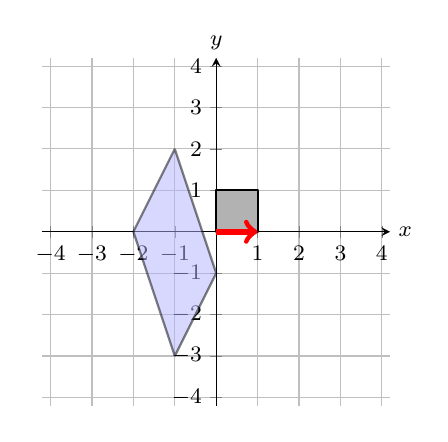
\begin{tikzpicture}
      \begin{axis}%
        [
	  xmin=-4.2,xmax=4.2,
          ymin=-4.2,ymax=4.2,
          xlabel=$x$,ylabel=$y$,
          axis lines=center,
          every axis y label/.style={at=(current axis.above origin),anchor=south},
          every axis x label/.style={at=(current axis.right of origin),anchor=west},
          clip=false,
	  grid =major,
          width=6cm,
          height=6cm,
          xtick={-4,-3,...,4},
          ytick={-4,-3,...,4},
	]
	\footnotesize
        \addplot[line join =bevel,black, thick,fill=black!30!white] coordinates{
          (0,0) (0,1) (1,1) (1,0) (0,0) (0,1)
          };
        \addplot [->,line width=2pt,color=red] coordinates{(0.,0.)  (1.,0.)};
        \addplot[line join =bevel,black, thick,fill=blue!30!white,opacity=0.5] coordinates{
		(0,-1) (-1,-3) (-2,0) (-1,2) (0,-1)
	};
        %\draw [->,line width=0.8pt,color=red] (0.,0.) -- (1.,0.);
      \end{axis}
    \end{tikzpicture}
    }
\choice{
  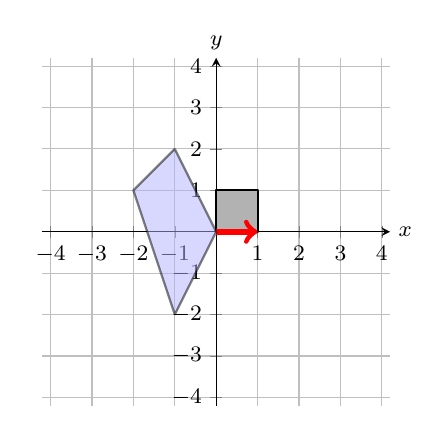
\begin{tikzpicture}
      \begin{axis}%
        [
	  xmin=-4.2,xmax=4.2,
          ymin=-4.2,ymax=4.2,
          xlabel=$x$,ylabel=$y$,
          axis lines=center,
          every axis y label/.style={at=(current axis.above origin),anchor=south},
          every axis x label/.style={at=(current axis.right of origin),anchor=west},
          clip=false,
	  grid =major,
          width=6cm,
          height=6cm,
          xtick={-4,-3,...,4},
          ytick={-4,-3,...,4},
	]
	\footnotesize
        \addplot[line join =bevel,black, thick,fill=black!30!white] coordinates{
          (0,0) (0,1) (1,1) (1,0) (0,0) (0,1)
          };
        \addplot [->,line width=2pt,color=red] coordinates{(0.,0.)  (1.,0.)};
        \addplot[line join =bevel,black, thick,fill=blue!30!white,opacity=0.5] coordinates{
		(0,0) (-1,-2) (-2,1) (-1,2) (0,0)
	};
        %\draw [->,line width=0.8pt,color=red] (0.,0.) -- (1.,0.);
      \end{axis}
    \end{tikzpicture}
    }
  \choice[correct]{ 
  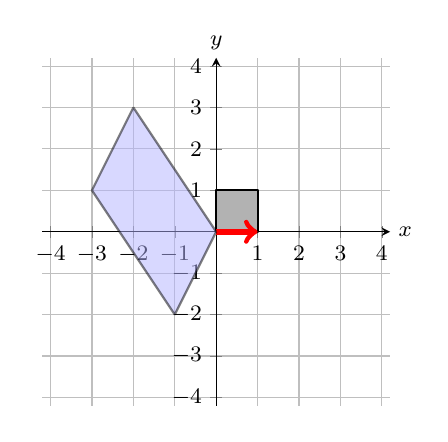
\begin{tikzpicture}
      \begin{axis}%
        [
	  xmin=-4.2,xmax=4.2,
          ymin=-4.2,ymax=4.2,
          xlabel=$x$,ylabel=$y$,
          axis lines=center,
          every axis y label/.style={at=(current axis.above origin),anchor=south},
          every axis x label/.style={at=(current axis.right of origin),anchor=west},
          clip=false,
	  grid =major,
          width=6cm,
          height=6cm,
          xtick={-4,-3,...,4},
          ytick={-4,-3,...,4},
	]
	\footnotesize
        \addplot[line join =bevel,black, thick,fill=black!30!white] coordinates{
          (0,0) (0,1) (1,1) (1,0) (0,0) (0,1)
          };
        \addplot [->,line width=2pt,color=red] coordinates{(0.,0.)  (1.,0.)};
        \addplot[line join =bevel,black, thick,fill=blue!30!white,opacity=0.5] coordinates{
		(0,0) (-1,-2) (-3,1) (-2,3) (0,0)
	};
        %\draw [->,line width=0.8pt,color=red] (0.,0.) -- (1.,0.);
      \end{axis}
    \end{tikzpicture}
    }
\end{multipleChoice}
\begin{question}
Correct!  Reasons for my choice:

Consider the vertices of the unit square:  
\begin{enumerate}
\item First vertex: The origin must be mapped to the $\answer[format=string]{origin}$.  
\item Second and third vertex: The images $Ae_1$ and $Ae_2$ must be vectors from the origin. 
\item Fourth vertex:  By linearity, $A(e_1+e_2) = Ae_1+Ae_2$, which means that the four vertex must be the vector sum of the first two.  By the $\answer[format=string]{parallelogram}$ rule, the vector sum $Ae_1+Ae_2$ is the diagonal of the $\answer[format=string]{parallelogram}$ formed by $Ae_1$ and $Ae_2$.  
\end{enumerate}
\begin{question}
Assuming the red arrow is mapped to the second quadrant, what is the matrix $A$? 
\[
A = \begin{bmatrix} \answer{-2} & \answer{-1} \\ \answer{3} & \answer{-2} \end{bmatrix}
\]
\end{question}
\end{question}
\end{question}
\end{document}
